\documentclass[stage]{tnreport}

\usepackage[utf8]{inputenc} 

\def\reportTitle{Mise en place d’un service de compilation/d’exécution isolé pour la plateforme PLM dédiée à l’apprentissage de la programmation} % Titre du mémoire
\def\reportLongTitle{Mise en place d’un service de compilation/d’exécution isolé pour la plateforme PLM dédiée à l’apprentissage de la programmation} % Titre plus long du mémoire

\def\reportAuthor{Tanguy GLOAGUEN}
\def\reportAuthorEmail{\email{tanguy.gloaguen@telecomnancy.eu}} % Courriel de l'élève

\def\reportSupervisor{Martin QUINSON, Gérald OSTER} % Prénom Nom de l'encadrant industriel

\def\reportCompany{LORIA} % Nom de l'entreprise d'accueil
\def\reportCompanyAddress{Campus Scientifique}  % Adresse de l'entreprise
\def\reportCompanyCity{54506, Nancy} % Adresse (cont.) de l'entreprise
\def\reportCompanyPhone{~} % Téléphone de l'entreprise
\def\reportCompanyLogoPath{figures/LORIA-logo.jpg} % Logo de l'entreprise

\def\place{Nancy} % Ville pour la signature pour l'engagement anti-plagiat
\def\date{\today} % Date pour la signature de l'engagement anti-plagiat

\def\reportProjectCustomer{}

\begin{document}

\maketitle
\pagenumbering{roman}

\insertAntiPlagiarismAgreement{GLOAGUEN, Tanguy}{31313847}

\cleardoublepage

\makesecondtitle

\section*{Remerciements}
\addcontentsline{toc}{chapter}{Remerciements}

{\em
Je tiens tout d'abord à remercier mes encadrants de stage, MM. Oster et Quinson, pour leur accueil au sein de leur équipe, leurs conseils et explications sur le système à étudier et le temps qu'ils ont accordé à l'étude des modèles proposés.

Je remercie également Matthieu Nicolas, qui m'a également encadré lors de ce stage, pour son aide précieuse sur les outils à utiliser, mais aussi pour son écoute et ses conseils quant aux méthodes de résolution des problèmes étudiés.

Enfin, je remercie mes collègues de bureau, MM. Bühler, Carpentier et Grguric, pour leurs aides sur la réalisation et pour l'ambiance agréable de travail.
}

\cleardoublepage

\renewcommand{\baselinestretch}{0.5}\normalsize
\tableofcontents
\renewcommand{\baselinestretch}{1.0}\normalsize
\cleardoublepage

\pagenumbering{arabic}
\setcounter{page}{1}

\chapter*{Introduction}

L'enseignement classique est celui généralement utilisé aujourd'hui, mais l'accés au public de l'informatique a permi de mettre en place des apprentissages plus automatisés : outils d'aide à l'enseignement, MOOC (cours en ligne) mais aussi logiciels d'apprentissage autonome.

Avec l'arrivée de nouveaux systèmes en autonomie permettant l'apprentissage de différentes matières, il était intéressant d'avoir un tel outil disponible pour l'informatique. L'outil le plus courant est bien sûr le tutoriel, mais parfois une approche plus interactive porte de meilleurs résultats sur les étudiants.

C'est dans ce contexte que se place la Programmer's Learning Machine : depuis 2007, cette application permet de standardiser les enseignements de base en programmation ainsi que d'aider les enseignants à évaluer les progrès des élèves.
La PLM a pour but d'enseigner les bases de la programmation et de fournir aux éudiants les meilleurs outils possibles pour apprendre à coder. Elle se base sur une dizaine d'univers différents, chacun apportant un angle ludique d'approche de problèmes informatiques.

En vue de moderniser le logiciel, il a été récemment proposé de transformer l'application PLM en un outil en ligne. Cette modification a entraîné des contraintes de sécurité, de puissance du matériel, de consommation mémoire et processeur des services et de mise à l'échelle supplémentaires qu'il a fallu résoudre.

Dans le cadre de ma formation d'ingénieur, il est demandé à la fin de la seconde année d'effectuer un stage dans le domaine de l'informatique. Ce stage a pour but de nous faire découvrir le travail dans l'informatique, la structure d'une entreprise et le travail sous contraintes économiques, humaines et temporelles.

J'ai effectué mon stage au Loria durant les mois de juin, juillet et août 2015, dans l'équipe Veridis et encadré par MM. Nicolas, Oster et Quinson. Dans le cadre de ce stage, je devais tenter d'apporter des solutions techniques aux problèmes rencontrés lors du passage d'une PLM en client lourd à un site internet.

Lors de ce stage, j'ai dû utiliser de nombreux outils et technologies qui seront présentées brièvement dans ce rapport. J'ai également mis en place un certain nombres d'architectures logicielles également présentées. Enfin, mes différentes contributions au projet seront expliquées.

Dans un premier temps, nous verrons le contexte du stage plus en détail : l'établissement d'accueil mais aussi la Programmer's Learning Machine en tant qu'application et qu'interface web.\\
Dans un second temps, nous verrons les objectifs du stage.\\
Puis, nous étudierons la réalisation de ces objectifs en tant que méthodologie, en tant qu'environnement et les résultats obtenus.\\
Enfin, nous ferons un bilan des résultats et une liste des améliorations prévues.



\chapter{Présentation}

\section{Le LORIA}

Le Laboratoire Lorrain de Recherche en Informatique et ses Applications (abrégé LORIA\cite{LR-WS}) est une Unité Mixe de Recherche créé en 1997 par association entre le CNRS (Centre National de la Recherche Scientifique), l'UL (Université de Lorraine) et l'INRIA (Institut National de Recherche en Informatique et Automatique).

La mission principale du LORIA est la recherche fondamentale et appliquée dans le cadre des sciences informatiques. Elle accueille un total de 450 personnes\footnote{chiffres 2014, http://www.loria.fr/rapports-activite-2/rapport-dactivite-2014}, réparties en 27 équipes sur 5 dépatements :
\begin{description}
	\item[Algorithmique, calcul, image et géométrie] \hfill \\
		Ce département de 6 équipes, dirigé par Sylvain Lazard, s'intéresse principalement aux algorithmes tout en gardant une différence sur les applications selon les équipes.
	\item[Méthodes formelles] \hfill \\
		 Ce département de 6 équipes, dirigé par Dominique Méry, développe des contributions aux logiques et théories de preuves. C'est dans ce département que se trouve VERIDIS et le projet PLM.
	\item[Réseaux, systèmes et services] \hfill \\
		 Département de 3 équipes dirigé par Ye-Quiong Song, il s'intéresse principalement aux problèmes issus des systèmes distribués et parallèles.
	\item[Traitement des langues et des connaissances] \hfill \\
		 Ce département de 8 équipes dirigé par Bruno Guillaume porte sur l'étude des langues naturelles, des conaissances et des documents.
	\item[Systèmes complexes et intelligence artificielle] \hfill \\
		 Département de 5 équipes dirigé par Bernard Girau, il s'occupe des méthodes d'apprentissage, d'analyse et de prise de décision rendus possibles par les intelligenes artificielles.
\end{description}

\clearpage

\begin{figure}[h]
	\centering
		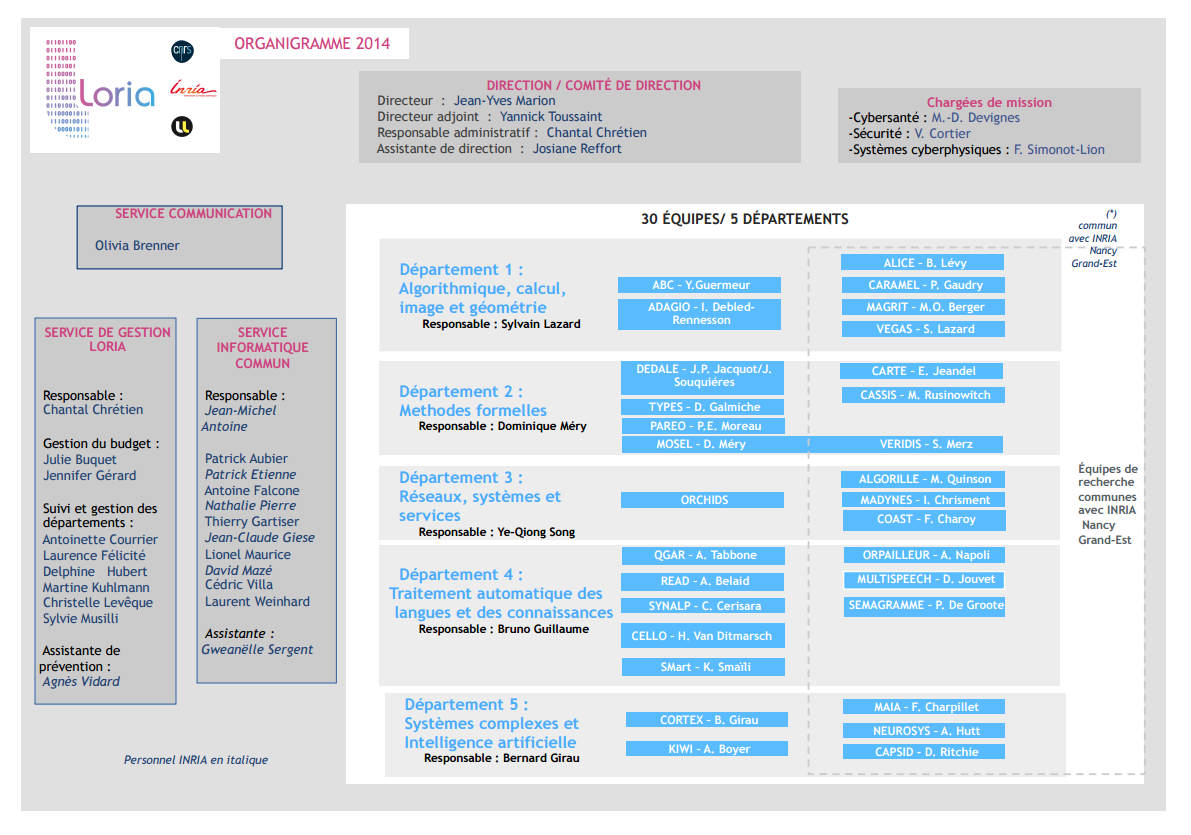
\includegraphics[width=0.9\textwidth]{figures/LORIA-organigramme}
	\caption{Organigramme du LORIA}
	\label{fig:organigramme}
\end{figure}

En tant qu'UMR, le LORIA possède sa propre administration. Un organigramme du LORIA est dispobible en \ref{fig:organigramme}\cite{LR-ORG}, présentant la structure interne. On y remarque que même si les différentes entités administratives sont bien définies, il n'y a pas de hiérarchie directe entre elles.


\section{La "Programmer's Learning Machine"}

Le projet "Programmer's Learning Machine" (abrégé PLM) est un projet commencé en 2007 par Martin Quinson et Gérald Oster.

Ce projet a pour but de fournir aux étudiants en informatique une plateforme d'initiation aux concepts de programmation basiques et avancés ainsi qu'un outil d'analyse et d'aide à la médiation pour l'enseignant.
La PLM est utilisée depuis à Telecom Nancy, et sert en première année à aider à la formation des nouveaux étudiants. Elle possède pour le moment plus de 200 exercices distincts portant sur divers sujet allant de l'introduction aux concepts de programmation à la récursivité ou aux tris.

\subsection{La PLM en tant qu'application lourde}

Dans sa forme originelle, la PLM était une application Java lourde écrite en Swing. L'utilisateur lançait le programme sur son ordinateur et obtenait des résultats. L'application lourde est aujourd'hui en version 2.6 et approche de la version 2.7.

La PLM est constituée d'exercices, regroupés en leçons et étendus sur différents univers : buggles, turmites, tortues mais aussi listes ou même simple tests sans interface particulière. Chaque exercice propose donc un scénario dans ces univers, présentant un nouveau concept à l'utilisateur.
Celui-ci doit alors trouver quel code permet de résoudre l'exercice en s'aidant de la démonstration, du texte de mission et de l'API\footnote{API : Application Program Interface, ensemble des commandes spécifiques au programme. Ici, il s'agit des commandes de l'univers.} du monde.
\begin{figure}[h]
	\centering
		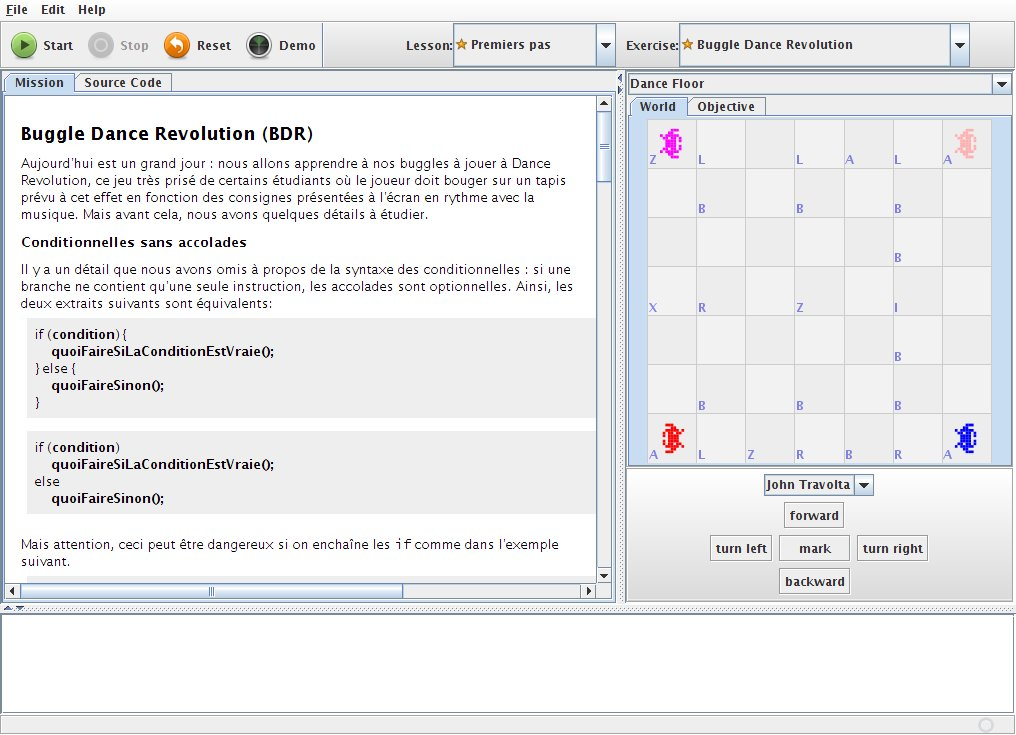
\includegraphics[width=0.9\textwidth]{figures/PLM-exercice1}
	\caption{Exemple d'exercice : Buggle Dance Revolution, portant sur la lecture d'informations et le pattern matching.}
	\label{fig:plmEx1}
\end{figure}

La PLM a été la cible de différents projets au cours du temps, de manière à ajouter des fonctionnalités : langage C, nouveaux exercices et nouvelles leçons et plus récemment aide spécifique à l'utilisateur et aux enseignants.

\subsection{Portage web de la PLM}

En plus des améliorations apportées à la PLM elle-même, il est question depuis décembre 2014 d'un portage AngularJS de l'application. Ce projet, nommé WebPLM, est principalement géré par Matthieu Nicolas.
La nouvelle architecture proposée est une interface client utilisant angular.js reliée via une WebSocket à un serveur web tournant sous Play Framework.

De cette manière, il serait en fait possible de centraliser les informations (ce qui permettrait un partage plus facile des améliorations) mais aussi pour permettre à terme de l'intégrer aux MOOC de programmation.
\begin{figure}[h]
	\centering
		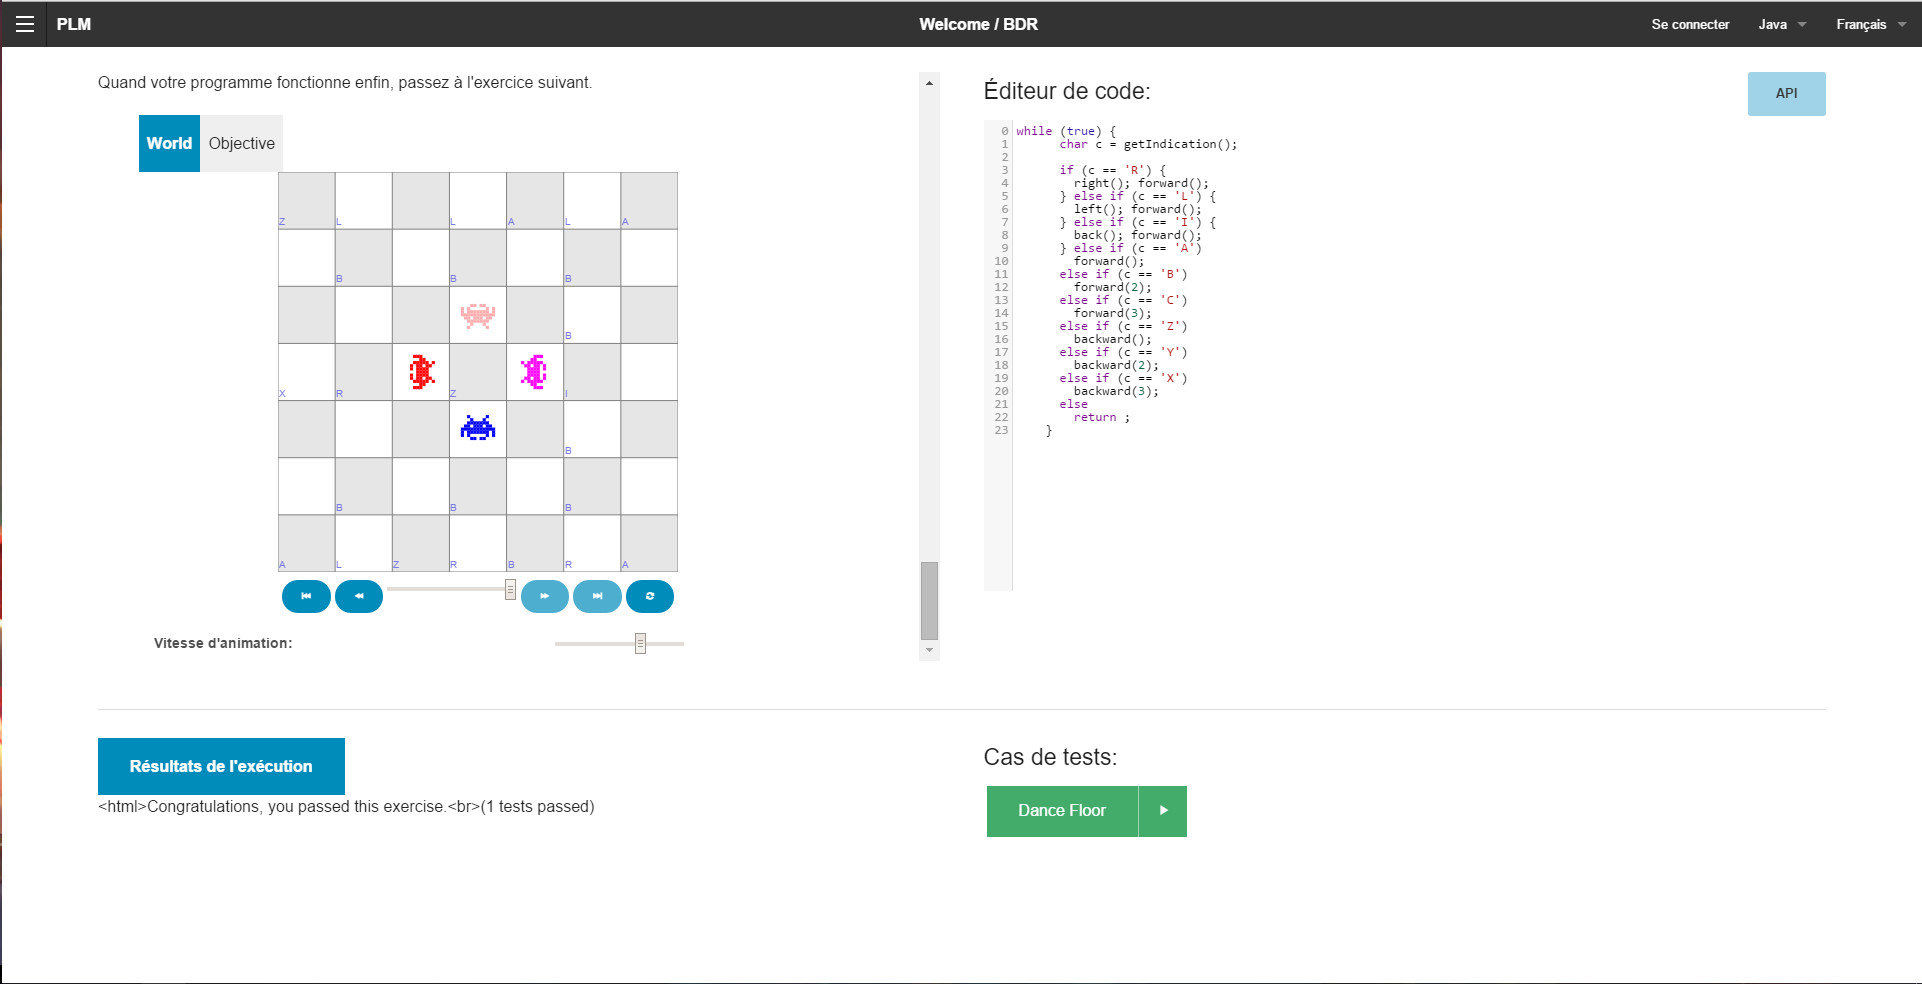
\includegraphics[width=0.9\textwidth]{figures/WebPLM-exercice1}
	\caption{Apparence de WebPLM, portage web de la PLM.}
	\label{fig:wplmEx1}
\end{figure}

Au début du stage, WebPLM était utilisable mais avait de fort problèmes de performance. Principalement, l'architecture utilisée était simpelment de prendre PLM et de relier l'ancienne interface graphique à une interface web.

Le portage web de PLM est aujourd'hui à un état utilisable, la plupart des exercices sont disponibles et les rares problèmes restants sont plus de l'ordre du confort visuel (problèmes d'affichage) ou de l'ordre de données non mises à jour.



\chapter{Problématique du stage}

\section{Contexte du stage}

Le portage web entamé récemment portait principalement sur l'interface client et l'utilisation de PLM, sans se soucier des problèmes de performance ou de sécurité :

Le principal désavantage du système était l'incapacité de celui-ci à supporter la charge de nombreux utilisateurs. En effet, la version originelle de WebPLM ne séparait aucun composant et l'exécution du code élève se faisait sur la même machine que celle qui fournisait les données à l'utilisateur. Le résultat est que dès qu'un seul utilisateur demandait de tester sa solution à un exercice, l'expérience de tous les autres utilisateurs était affectée.

Le second désavantage était le problème de séurité. Il n'y avait aucune restriction aux actions de l'utilisateur sur le programme. Le résultat est que l'utilisateur avait accès à la machine via le logiciel aussi sûrement que s'il était devant un clavier. Cela posait de nombreux problèmes quant aux personnes mal intentionnées, qui avaient accès à un poste informatique sur lesquels leurs actions n'étaient pas reliées à leur identité.

Le projet ayant aujourd'hui atteint un niveau ou son déploiement est envisageable, il est nécessaire d'adresser ces deux problèmes.

Pour palier à cela, MM. Quinson, Oster et Nicolas ont envisagé de séparer les deux composantes principales de la PLM : l'environnement d'exécution des exercices et l'environnement d'évolution de l'élève.
Cette solution permettrait donc d'isoler l'exécution dans des environnements contrôlés et dont la performance peut être mise à l'échelle.

Cependant, la PLM n'a pas été prévue pour séparer ces deux fonctions, il fallait donc comprendre le code d'origine et mettre en place une stratégie pour le séparer.

Après avoir préparé cette stratégie, il fallait la mettre en place de manière non seulement à pouvoir utiliser WebPLM en enseigenement mais aussi prévoir les possibilités d'améliorations et d'expansion du logiciel. Cela signifie architecture stable et une mise à l'échelle possible.

\section{Objectifs du stage}

Ce stage avait donc pour objectif de séparer les composantes de compilation/exécution de code élève et de gestion du progrès de l'élève.

Les objectifs du stage ont donc été de :
\begin{itemize}
	\item Identifier les composantes d'exécution et de gestion de l'élève dans la PLM.
	\item Créer un outil d'exécution de code
	\item Utiliser cet outil lors de la demande d'exécution de code
	\item Rendre l'outil sécurisé et distribuable.
	\item Améliorer la PLM pour retirer les composantes inutiles
\end{itemize}

L'état final attendu était un site internet pouvant supporter une charge importante (objectif de 90 nouveaux étudiants à la rentrée 2015-2016) et pour lesquels les améliorations seraient assez faciles à ajouter.

Les pistes proposées par les encadrants de stages étaient de :
\begin{itemize}
	\item Utiliser une queue de message pour stocker les informations de compilation
	\item Utiliser la technologie Docker\cite{DCK-WS} pour rendre le système distribuable.
	\item Utiliser Docker + un SecurityManager\footnote{java.security.SecurityManager est un composant Java pour gérer les autorisations des logiciels} pour sécuriser l'environnement d'exécution.
\end{itemize}

Pour réaliser ces objectifs, il fallait étudier et trouver différentes technologies et différents modèles correspondant à ces pistes fournies.

\chapter{Réalisation}
\section{Environnement de réalisation}

La réalisation s'est principalement faite sur un environnement de développement Windows et un environnement d'exécution Linux.

Les technologies utilisées étaient :
\begin{description}
	\item[Docker] \hfill \\
		Docker est une technologie de gestion d'applications distribuées. Le principe est de créer des images de machines virtuelles (appelées images docker) qui, une fois lancées, sont directement utilisables avec tous logiciels lancés. \\
		Une telle technologie a pour effet de rendre presque trivial la mise en production et la mise à l'échelle des environnements.
	\item[RabbitMQ] \hfill \\
		Rabbit MQ\cite{RMQ-WS} est un gestionnaire de queue de message. Une queue de message est un  système permettant de stocker temporairement des données par "bloc". On peut se connecter à cette queue de message pour y déposer des blocs ou en demander un. \\
		L'idée est que les clients ne s'intéressent pas à qui traite les mesages, juste à ce qu'il soit traité.
	\item[Play Framework] \hfill \\
		Play Framework\cite{PFM-WS} est une application de déploiement de serveur web. Il permet d'installer rapidement un environnement web basé sur une JVM (java ou scala). C'est le système choisi pour développer la version web de la PLM.
\end{description}

En plus de ces technologies, il était nécessaire de créer le modèle de l'application. Il a donc été nécessaire d'appliquer différents designs patterns.

\section{Méthode de réalisation}

\subsection{Modèle global envisagé}

Le modèle de WebPLM au début du stage était assez proche de celui de PLM. En effet, WebPLM "contenait" dans son intégralité Game, le composant principal de PLM. On obtenait donc les figures \ref{fig:plmUP1} et \ref{fig:wplmUP1} suivantes :
\begin{figure}[h]
	\centering
		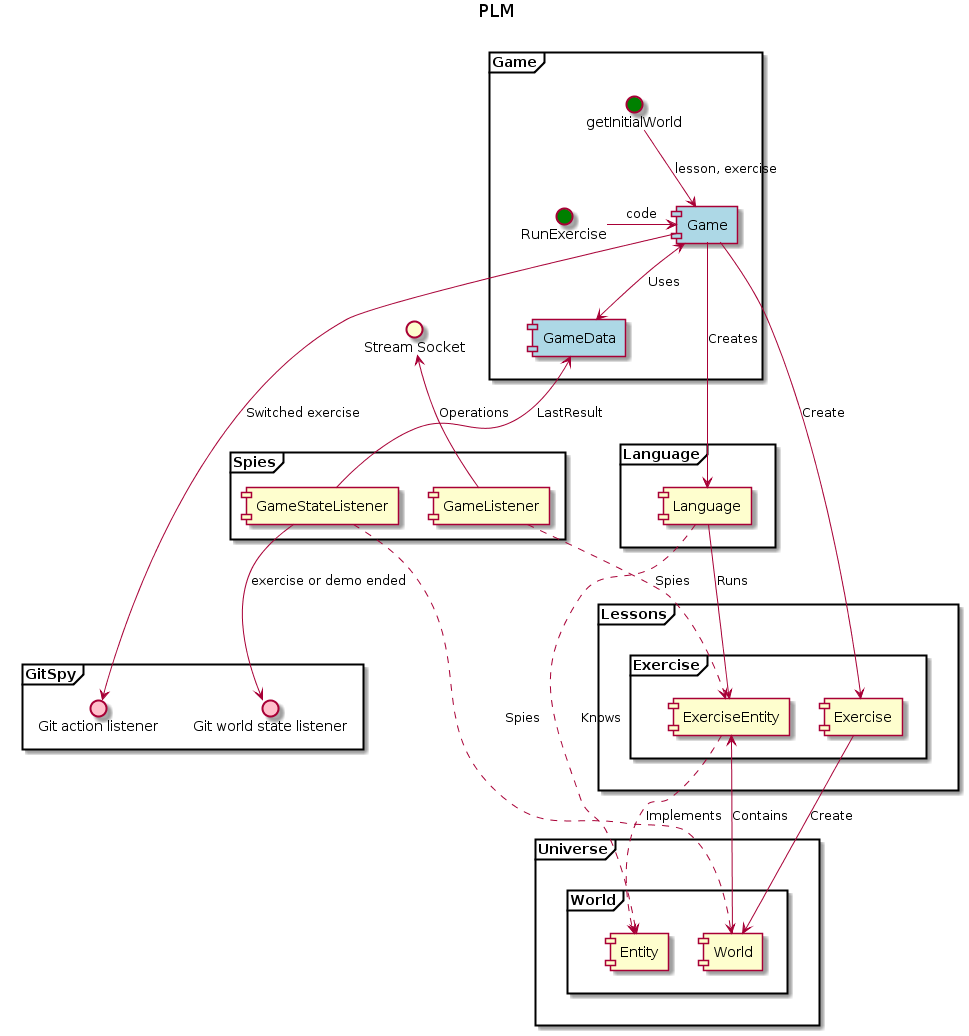
\includegraphics[width=0.5\textwidth]{figures/PLM-uml-cp1}
	\caption{Représentation complète de PLM à son exécution}
	\label{fig:plmUP1}
\end{figure}
\begin{figure}[h]
	\centering
		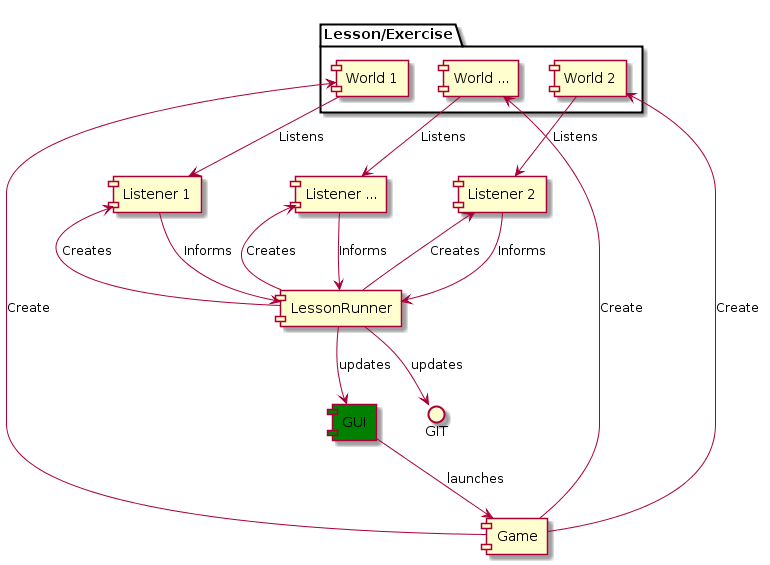
\includegraphics[width=0.7\textwidth]{figures/WebPLM-uml-cp1}
	\caption{Représentation simplifiée de WebPLM au début du stage}
	\label{fig:wplmUP1}
\end{figure}

Le but de l'amélioration est de séparer les appels de compilation du serveur. Pour commencer, la modélisation du problème en diagramme de séquence a été réalisée (fig \ref{fig:wplmUS1}).
\begin{figure}[h]
	\centering
		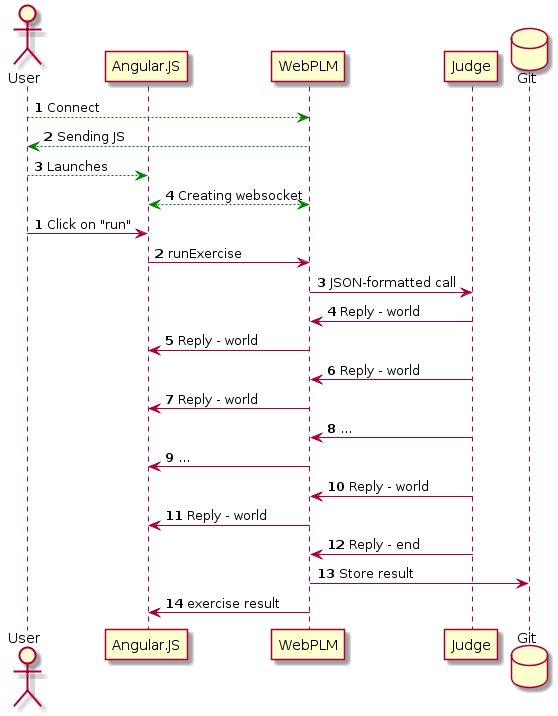
\includegraphics[width=0.4\textwidth]{figures/WebPLM-uml-Seq1}
	\caption{Diagramme de séquence du problème. En vert est l'étape de connexion, déjà créée dans WebPLM au moment du stage}
	\label{fig:wplmUS1}
\end{figure}

A partir de ce diagramme de séquence, nous avons pu d'abord identifier les différentes composantes de WebPLM qu'il était nécessaire de séparer. Ce qui est noté "Judge" sur ce schéma est donc la nouvelle composante qu'il fallait créer.

Cette composante devait contenir tous les procédés de compilation mais aussi l'environnement nécessaire pour faire évoluer l'univers\footnote{Dans PLM, un univers (plm.universe) est un ensemble représentant informatiquement ce qui est affiché à l'écran. Un exercice est donc un scénario qui se base sur un univers.} affiché à l'élève et les données sur l'execice courant.

En plus de cette composante de compilation, il a fallu définir un protocole avec lequel faire communiquer la composante de compilation et la composante de gestion de l'élève. Pour cela, il fallait choisir une technologie appropriée. 

Il a été envisagé dans un premier temps d'effectuer les appels de compilation par des appels RMI\footnote{RMI : Remote Method Invocation est une technologie génralement utilisée dans le cas où on veut qu'un système externe fasse une opération sans le considérer comme système externe.}.
Cependant, la technologie RMI de Java n'était pas prévue pour récupérer plus d'un résultat, ce qui posait problème vu que le juge est supposé informer des changement d'états du monde au fur et à mesure de son exécution.

Le modèle envisagé a donc été dans un second temps un gestionnaire de queue de messages, RabbitMQ.

Une queue de message permet à la fois de gérer des données de façon indépendante de l'architecture logicielle et de ne poser aucune contrainte sur le format de retour. Cela permet donc de contourner le problème posé précédemment de plusieur "réponses" pour une seule requête.

Le modèle étudié partait sur une file d'attente contenant des demandes de compilation ainsi que de files de retours permettant d'envoyer les évolutions et résultats de l'exécution du code élève.

C'est sur ce second modèle utilisant RabbitMQ que je me suis engagé lors de ce stage.

\subsection{Création des juges}

Les juges sont de simples conteneurs de la version de PLM déjà présente dans WebPLM. Cependant, ils possèdent une interface leur permettant de communiquer avec une queue de message.

L'idée derrière les juges est de lancer un environnement de simulation PLM, de le forcer dans le "bon" état pour l'exercice demandé et de fournir le code élève à PLM. Les modifications à apporter au logiciel étaient donc minimes pour atteindre des résultats probants. De plus, il fallait une interface d'attente de messages et de lecture de ces messages. Enfin, il fallait redémarrer l'environnement PLM à chaque fin de simulation pour éviter la propagation de modifications potentielles dûes aux élèves à d'autres exécutions.

En plus de la création des juges, il a été mis en place un environnement pour tester leur fonctionnement. Cela permet, en plus des tests d'intégration déjà présent dans la PLM, de tester le fonctionnement des juges eux-même en lançant différents codes. Ces tests sont toujours présents dans la version actuelle des juges.

Cette étape a duré approximativement deux jours, terminée le 26-06.

\subsection{Utilisation des juges}

Dans un second temps, il était nécessaire de refabriquer l'étape de compilation de WebPLM. Pour cela, il a fallu dans un premier temps écrire la structure d'appel et de récupération depuis la queue de message, puis de reformater le code de manière à le rendre utilisable.

\subsubsection{Système de base}
Tout d'abord, il a fallu écrire un système de base permettant à WebPLM d'utiliser la message queue pour gérer les appels de compilation et d'en récupérer les résultats pour les transmettre au client.

Pour cela l'approche logicielle a été de créer une autre interface côté serveur, utilisant l'API de RabbitMQ pour lancer de nouveaux appels de compilation.

L'étape d'écriture du code a pris environ 3 jours, terminée le 01-07. A ce moment, WebPLM utilisait déjà des juges parallélisables pour la compilation.

\subsubsection{Stockage du résultat}
Il fallait ensuite réécrire les appels au gestionnaire GIT de manière à enregistrer la progression de l'élève ainsi que son code. Il a été nécessaire d'extraire le gestionnaire du Game toujours présent dans WebPLM et de l'utiliser à partir de là.

Lorsqu'un élève réussit ou échoue un exercice, le code qu'il a proposé ainsi que les résultats qu'il a obtenus sont stockés dans un gestionnaire Git local. Le but de ce gestionnaire est de pouvoir remettre l'élève au même niveau de progression après une déconnexion amis aussi de pouvoir faire des études sur les données fournies par les élèves. Cela entre dans le cadre de plusieurs autres projets en lien avec la PLM.

Cette étape a duré deux autres jours, terminée le 03-07.

\subsubsection{Analyses de performances, limites d'exécution, arrêt automatique}
Enfin, il a fallu tester les performances et adapter le résultat en conséquence.

La première version avait d'énormes problèmes de performance. Cela était dû au fait que la queue de messages contenait un message par opération du monde, message générés en parallèle qui plus est.
J'ai donc mis en place un accumulateur au niveau des listeners (cf figure \ref{fig:wplmUP1}) pour n'envoyer qu'une opération toutes les 500ms. Cela a résolu le problème de performance de base.

Il y avait également un problème de stabilité lors de compilations se terminant en boucle infinie. Pour gérer cela, il a été mis en place un système de sémaphore avec tentative d'acquisition pendant X secondes (X valait 30s, puis 15, puis 10 au fur et à mesure du projet), sémaphore réveillée par les listeners lors de la fin d'exécution.

Le résultat final était donc une version de PLM stable, décrite en figure \ref{fig:wplmUP2}.
\begin{figure}[h]
	\centering
		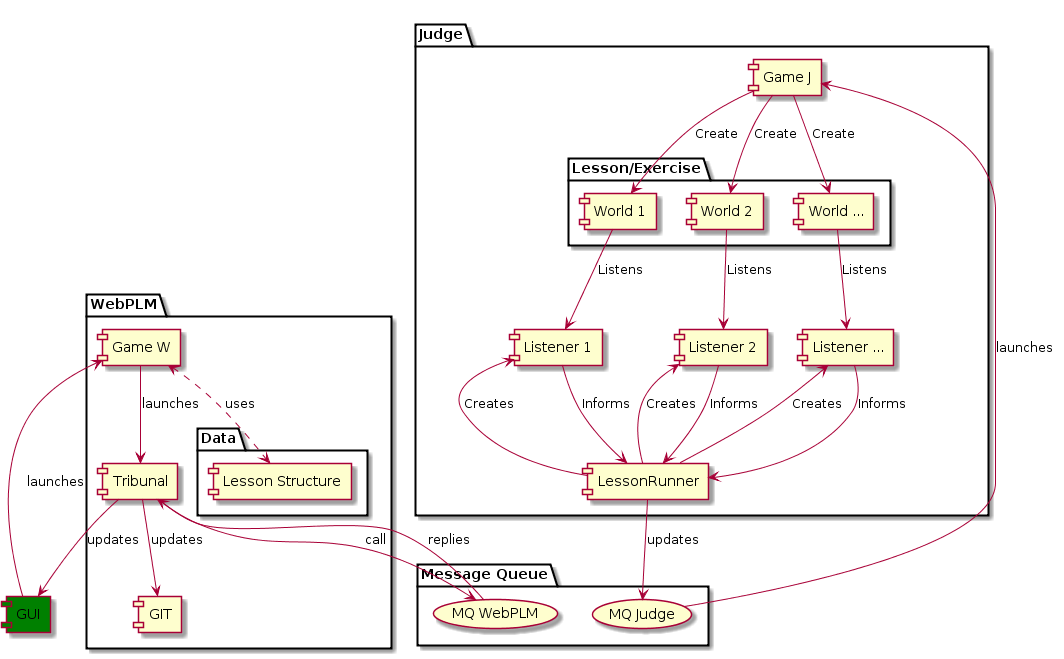
\includegraphics[width=0.7\textwidth]{figures/WebPLM-uml-cp2}
	\caption{Structure simplifiée de WebPLM et juges à la fin de l'étape de création des juges.}
	\label{fig:wplmUP2}
\end{figure}

\subsection{Etude d'un mode débug}

Pendant les semaines suivantes du stage, il a été question d'un mode "débug" de PLM. Ce mode débug devait permettre aux élèves d'avoir un aperçu de l'évolution de leurs variables et au système d'enseignement de détecter des schémas plus précis où l'élève resterait bloqué.

Différentes solutions ont été étudiées au cours du stage, en particulier la librairie JDI\footnote{com.sun.jdi est une librairie prévue pour analyser une JVM depuis une autre JVM} de Java pour détecter les modifications sur l'autre machine. Cependant, ce projet n'a jamais eu la priorité qu'il aurait fallu pour le mener à terme.

\subsection{Utilisation de Docker}

Après avoir modifié WebPLM pour se comporter en deux parties, il a été nécessaire d'adapter ces deux parties pour qu'elles puissent être utilisées dans des containers Docker.

L'idée était de pouvoir utiliser un container par juge lancé, de manière à posséder plusieurs instances de juges indépendantes et séparées. En utilisant de plus les outils fournis en parallèle avec Docker (en particulier docker-compose), il est possible de changer le nombre de juges actifs en une simple commande.

Le second intérêt de l'utilisation de Docker est que la création des containers est une tâche indépendante de leur utilisation. Cela permet d'avoir un environnement permettant la génération sur une seule machine physique et de déployer le système sur une architecture combinée simplement, sans problèmes de compatibilité.

Les principaux défis de cette étape n'ont pas été la réalisation elle-même mais la compréhension des différents problèmes rencontrés.

\begin{description}
	\item[Interaction entre Docker et Maven] \hfill \\
		Docker et Maven sont deux outils ayant des propriétés similaires : la centralisation des données en vue d'une utilisation déployable facilement. Le principal souci rencontré est lors de la génération des images Docker, Maven devant télécharger à chaque fois l'intégralité des composants.
		\hfill \\
		Le résultat était une compilation à réussite aléatoire. \hfill \\
		Nous avons dû compiler\footnote{Cette compilation se fait en utilisant la commande "activator stage". Le comportement habituel de Play Framework est de recompiler au fur et à mesure si on utilise "activator start/run"} le serveur Play Framework en dehors du docker, pour éviter de devoir retélécharger les dépendances à chaque fois.
	\item[Déploiement de RabbitMQ et utilisations de variables internes] \hfill \\
		Les différents composants de WebPLM avaient tous besoin d'un outil commun : la conaissance de l'adresse de la Message Queue. Il a fallu modifier WebPLM et les juges de manière à pouvoir récupérer ces informations automatiquement.
\end{description}

Cette étape aura duré du 09/07 au 16/07.

\subsection{Documentation du code existant}

Une phase de documentation et de refactoring a alors pris place. Maintenant que tous les composants étaient mis en place, il était possible de refabriquer les structures de données de manière à les adapter au mieux aux tâches qu'elles devaient réoudre.
Une javadoc des ajouts déjà effectués à été également réalisée de manière à rendre plus facile toute modification subséquente du code.

Cette étape s'est étendue sur les 20 et 21 juillet.

\subsection{Ajout d'opérations de logging}

Une étape de l'amélioration du projet WebPLM a été de rajouter l'affichage du canal de sortie standard sur l'écran de l'utilisateur. Pour cela, il a fallu capturer toutes les données de sortie standard et les rediriger en tant qu'opérations vers l'utilisateur. Il a également fallu recréer un canal spécifque permettant aux logs de l'application de tout de même apparaître sur la sortie standard.

Cette étape a pris place les 22/07 et 23/07.

\subsection{Standardisation des données}

Un problème assez particulier nous est apparu. Pour certains mondes, malgré que le code soumis à l'utilisateur corresponde à la solution de l'exercice et que le juge validait le résultat, la représentation du monde affiché ne correspondait pas aux résultats attendus.

Comme dit précéemment, un exercice est d'un point de vue logiciel un scénario dans un univers. En tant que tel, les données d'un exercice dépend de la structure de l'univers et de son initialisation.

Il s'avère que la génération de certains univers (par exemple, les listes lors des tris) était aléatoire, ce qui provoquait une discordance entre les actions calculées à partir du monde du juge et celles appliquées sur le monde affiché. Il a donc fallu "standardiser" les univers, s'arranger pour qu'ils aient tous les mêmes valeurs quelque soit l'environnement.

Pour cela, il a été appliqué une méthode simple : les fonctions aléatoires ont vu leur "seed" se faire fixer au même nombre. Selon la Javadoc, les résultats sont donc maintenant strictement identiques quelque soit le système utilisé.

Cela a été effectué le 24/07.

\subsection{Pré-génération des données}

En vue du passage a une version de WebPLM (côté serveur) sans la composante PLM, il fallait générer les données nécessaires (structures des execices, état initial des mondes, démonstrations) et les stocker de façon statique avant de pouvoir juste supprimer Game.

Pour arriver à ce résultat, il a fallu modifier un juge pour lui faire parcourir tous les exercices et, pour chacun, générer la démonstration et l'état initial.

La méthode utlisée s'est faite en plusieurs étapes.

Dans un premier temps, il a fallu convertir les fonctions permettant de transformer les données du logiciel en données compréhensibles côté utilisateur. Ces fonctions, écrites en Scala pour le serveur Play Framework, ont dû être réécrites en Java pour le juge modifié.

Ensuite, il a fallu créer des fonctions permettant de stocker le résultat. L'idée étant d'utiliser le format JSON déjà présent côté serveur Play, il suffisait juste d'utiliser une librairie JSON et les outils de base pour écrire du texte dans un fichier.

Enfin, il a fallu établir une méthode de parcours des données permettant de faire l'action sur tous les exercices de toutes les leçons. Pour cela, il a fallu récupérer la liste des exercices et appliquer les méthodes de conversion et de stockage sur chacune des démonstrations.

Cette étape a été effectuée du 27/07 au 05/08

\subsection{Nettoyage de la PLM}

La dernière étape de ce stage a été de tenter de retirer PLM (en particulier Game) de WebPLM. Pour cela, il fallait étudier les différentes composantes utiles de PLM, les réécrire au mieux pour Play Framework (en Scala) et résoudre le diférents problèmes de taille mémoire et de concurrence qui apparaissaient.

Au début de cette étape, la structure de PLM était celle présentée en figure \ref{fig:wplmUP3}.
\begin{figure}[h!]
	\centering
		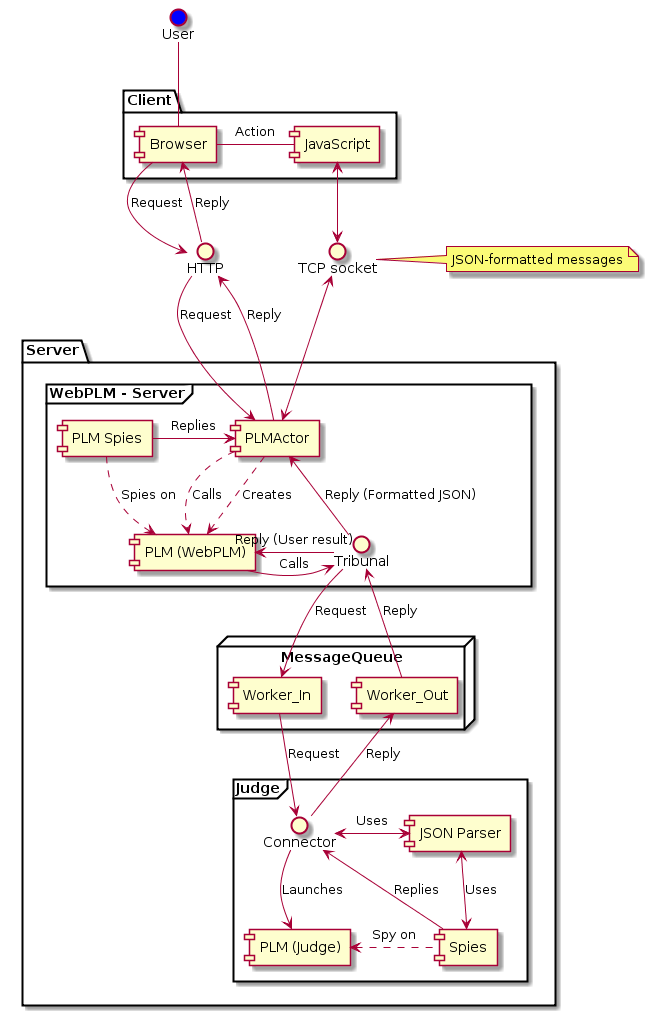
\includegraphics[width=0.5\textwidth]{figures/WebPLM-uml-cp3}
	\caption{Structure de WebPLM au début du nettoyage}
	\label{fig:wplmUP3}
\end{figure}

Le but était d'obtenir une structure telle que celle en \ref{fig:wplmUP4}.

\begin{figure}[h]
	\centering
		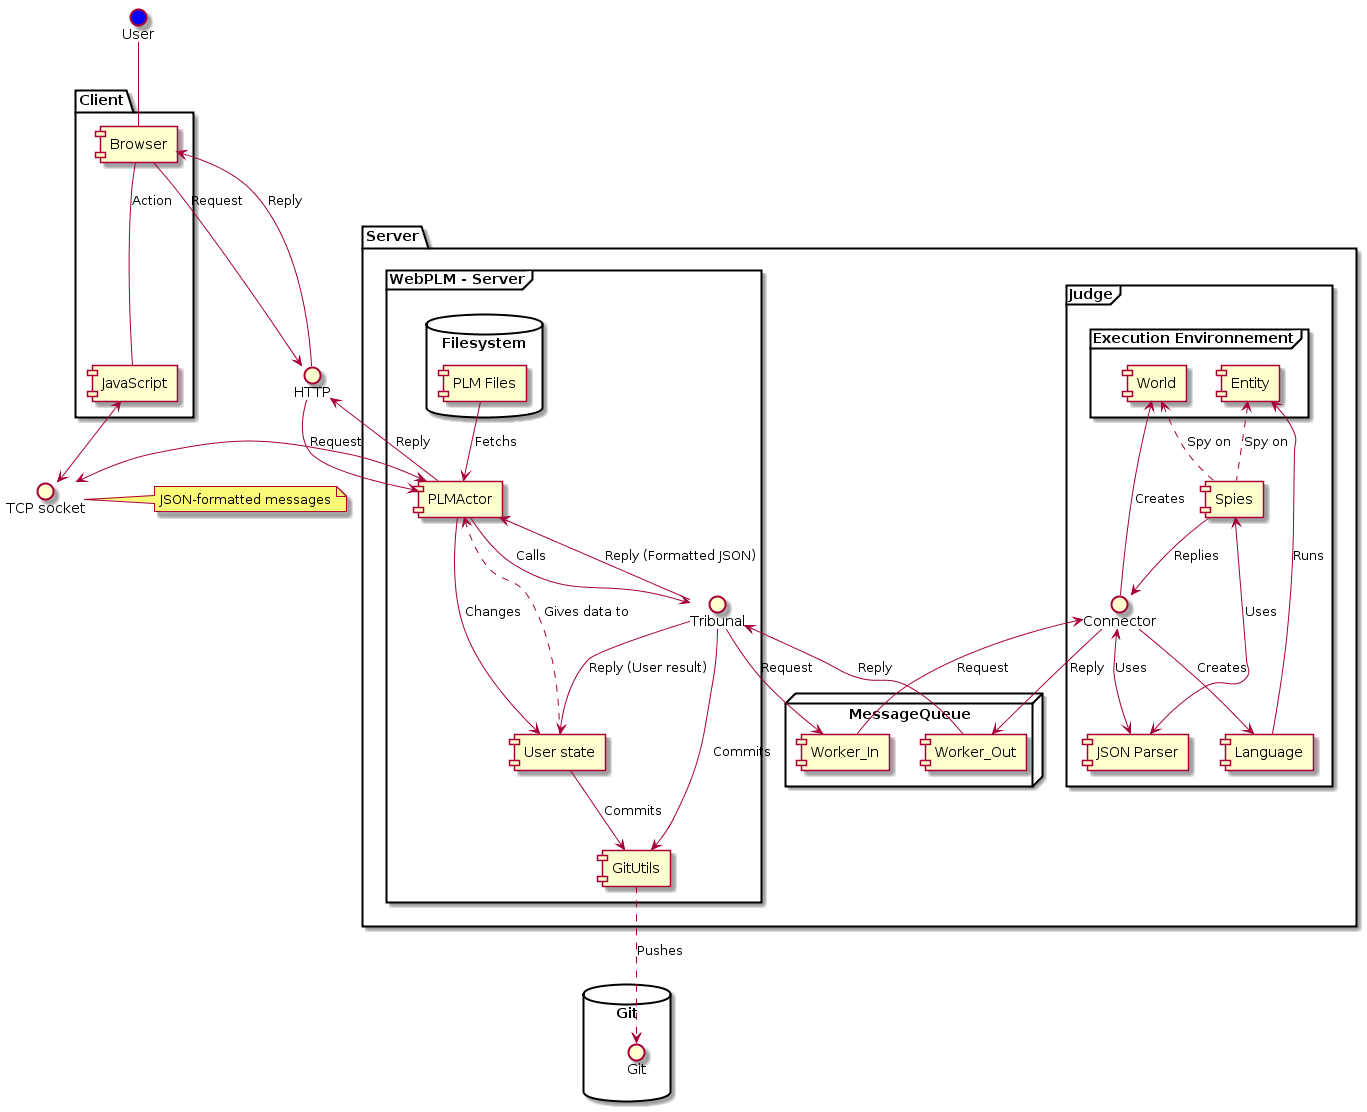
\includegraphics[width=0.9\textwidth]{figures/WebPLM-uml-cp4}
	\caption{Structure finale idéale de WebPLM.}
	\label{fig:wplmUP4}
\end{figure}

Les principales étapes de ce nettoyage ont été de retirer la composante de lecure de données, les missions (textes d'informations sur les exercices) et les APIs (textes d'informations sur les mondes), la composante de localisation ainsi que celle de gestion du langage de programmation. Il a fallu également convertir les fonctions de génération en fonction de lecture ou d'exposition : les démonstrations sont par exemple pré-générées et exposées en tant que fichiers par le serveur et c'est le client qui va les chercher pour les afficher, ce qui améliore énormément les performances du serveur.

Le retrait de Game demande de recoder une grosse partie des interfaces logicielles utilisées par PLM et de les intégrer directement au serveur. Le résultat est que le modèle du serveur a été transformé, passant d'un modèle où l'on appelle Game comme interface à un modèle ou chaque action es codée indépendamment. Cela rend à la fois l'utilisation du système mais aussi son amélioration plus simple que le modèle de base utilisé.

Cependant, il reste un grand nombre de fonctions non converties : gestion du changement de leçon, d'exercice et de langue (naturelle/programmation), sauvegarde des données sur le gestionnaire GIT.

Cette tâche, commencée le 06/08, continue encore aujourd'hui.

\subsection{Mise en place d'un Security Manager}

Vers la fin de la période, nous nous sommes rendu compte que de nombreuses failles de sécurité que Docker était censé résoudre ne l'étaient en fait pas : accès à l'internet depuis un container, surcharge du processeur et surcharge du disque dur.

Pour résoudre certains de ces problèmes, nous avons utilisé un outil mis à disposition par Java, le Security Manager. Il permet de limiter les actions possibles pour chaque composante de l'application.

La mise en place du SeurityManager a permis de limiter les actions de l'utilisateur à la stricte utilisation des commandes disponibles dans l'application ainsi que d'empêcher l'utilisateur d'utiliser des commandes de communication web ou de création de fichiers. Les problèmes de sécurité restants (charge CPU, principalement) sont hors de portée de ce système.



\chapter{Résultats}

\section{Bilan}

\subsection{Modèle final}

Le modèle final de WebPLM est donc celui présenté en \ref{fig:wplmUP5}
\begin{figure}[h]
	\centering
		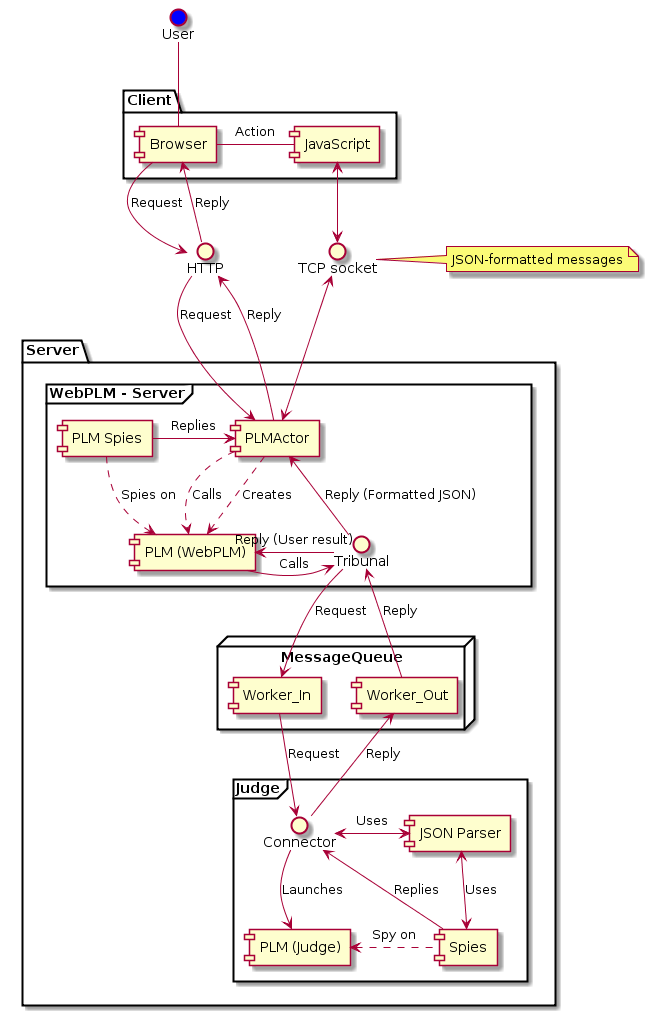
\includegraphics[width=0.6\textwidth]{figures/WebPLM-uml-cp3}
	\caption{Structure de WebPLM a la fin du stage.}
	\label{fig:wplmUP5}
\end{figure}

Cette structure est la même qu'avant le nettoyage. En effet, le nettoyage n'est pas terminé. Cependant, cette version apporte bien des améliorations par rapport à la version de WebPLM présente à l'origine.

La version actuelle est plus sécurisée. En effet, chaque composante du système est séparée dans un container différent.

De plus, cette version est plus simple à mettre à l'échelle : les composants sont dupliquables, en particulier le Juge qui est prévu spécifiquement pour être dupliqué.

 \subsection{Apports}

Un certain nombre d'apports ont été faits à PLM au cours de ce stage.

Dans un premier temps, l'objectif principal de séparer les composantes d'exécution et de gestion est accompli. En plus de juste être séparé, chaque composant peut être mis à l'échelle indépendamment des autres et peut même être lancé sur des machines physiques différentes.

Des fonctions utilitaires ont été rajoutées, telles que : gestion de la sortie d'affichage standard, suppression des composantes aléatoires des exercices. Ces fonctions amélioreront l'expérience de l'utlisateur et permettront une plus grande consistence dans l'aalyse et la récupération des résultats.

De gros progrès ont été également apportés sur l'étape de retrait de PLM depuis WebPLM. Même si cette partie n'a pas été terminée, l'avancement et la documentation permettra à cette étape d'être terminée probablement pour fin 2015.

Enfin, un travail de défrichage a été fait sur le mode débug, qui permettra de nouveaux outils sur le logiciel.

\subsection{Produit final}

A la fin de mon stage, la version de WebPLM est une version bien plus résistante à la charge et aux erreurs ou malices des utilisateurs que la version d'origine.

Des tests sur la version de production laissent penser que la nouvelle architecture pourra supporter les demandes objectifs de ce stage : une charge de 80 utilisateurs est quelque chose d'envisageable.

Les réalisations lors de ce stage ont été conformes aux objectifs du stage. Aujourd'hui, la version de production de PLM utilise le système séparé mis en place lors de ce stage, y compris les diverses améliorations apportées.

De plus, le produit de ce stage est une architecture qui peut être distribuée sur plusieurs machines. Ce n'était pas un objectif obligatoire du stage mais cela permet plus simplement de gérer de grosses puissances de calculs.

\section{Améliorations possibles}

Cependant, une partie importante du travail effectué est encore inachevé.

Les améliorations prévues aujourd'hui sont donc celles abordées lors de ce stage : la suppression de PLM de l'ensemble du serveur et la mise en place d'un système de débug pour avoir plus d'informations sur l'exécution.

Il y a également certains points, non abordés pendant ce stage, qui sont encore prévus : la suppression de la composante PLM des juges et l'envoi direct de données nécessaires à la compilation.



\chapter*{Conclusion}

Lors de ce stage, j'ai été confronté à plusieurs problèmes inédits.

\begin{itemize}
	\item Tout d'abord, j'ai dû ajouter des fonctionnalités à un logiciel déjà existant depuis plusieurs années. Il a fallu que j'acquière la mentalité lors de sa création, que je puisse manipuler ses composants et que je comprenne sa structure lors de mon stage.
	\item J'ai également dû m'intégrer à une équipe active sur un projet en pleine expansion. Pour cela, j'ai eu à maîtriser de nouveaux outils de gestion de projet, à intégrer mes rendus de projets dans le planning général de l'équipe et à présenter mes améliorations explicitement au chef de projet avant qu'elles puissent être utilisés dans le logiciel final.
	\item J'ai enfin eu à créer un système qui sera amélioré par d'autres après moi. C'est une expérience nouvelle, qui m'a forcé à utiliser non seulement des outils et techniques standardisées mais aussi à créer une documentation quant à l'utilisation future de mes contributions.
\end{itemize}

Mes contributions lors de ce stage ont également été très bénéfiques pour le projet.

\begin{itemize}
	\item D'une part, la création d'une architecture distribuée assure la pérénité de l'application au vu des futures améliorations technologiques sur l'architecture matérielle proposée.
	\item De plus, les nouvelles structures permettent d'intégrer aisément de nouveaux modules au projet. D'une manière générale, l'ajout de donénes au programme est resté le même. Cependant, l'ajout de fonctionnalités est très différent de ce qu'il était avant, plus séparé entre différentes composantes.
	\item Enfin, 
\end{itemize}



La transformation de PLM en une application web est une étape importante de la PLM : l'outil pourrait devenir bien plus utilisé, non seulement dans l'enseignement en informatique mais peut-être également dans l'enseignement général.

\cleardoublepage

\begin{thebibliography}{5}

\bibitem{DCK-WS}
	"Docker",
	\emph{Docker - Build, Ship and Run Any App, Anywhere}, \hfill \\
	\url{https://www.docker.com/}.

\bibitem{LR-WS}
	"LORIA",
	\emph{Site officiel du LORIA}, \hfill \\
	\url{http://www.loria.fr/}.

\bibitem{LR-ORG}
	"Organigramme",
	\emph{Organigamme du LORIA}, \hfill \\
	\url{http://www.loria.fr/le-loria-1/organisation/organigramme}.

\bibitem{PFM-WS}
	"Play Framework",
	\emph{Play Framework - Build Modern \& Scalable Web Apps with Java and Scala}, \hfill \\
	\url{https://www.playframework.com/}.

\bibitem{RMQ-WS}
	"RabbitMQ",
	\emph{RabbitMQ, messaging that just works}, \hfill \\
	\url{https://www.rabbitmq.com/}.

\end{thebibliography}

\cleardoublepage
\thispagestyle{empty}

\section*{Résumé}
\addcontentsline{toc}{chapter}{Résumé}
Le projet PLM (Programmer's Learning Machine) a pour but d'enseigner l'informatique aux personnes qui l'utilisent. Dans le cadre du développement web de cette application utilisant Play Framework et Angular.js, il a fallu mettre en place un système séparant l'exécution de code de la gestion des utilisateurs. Pour cela, nous avons implémenté un système de queue de message entre composantes d'exécution et un serveur de gestion. Ces composantes d'exécution sont dans des containers Docker et peuvent être mises à l'échelle.

{\bf Mots-clés :} Apprentissage, Docker, queue de messages, RabbitMQ, Play Framework, Angular.js


\section*{Abstract}
\addcontentsline{toc}{chapter}{Abstract}
The Programmer's Learning Machine (PLM) project is aiming at teaching computer science to its users. While switching this application to a Play Framework and Angular.js web app, we had to create a system to split code execution and user management. We implemented a message queue system between compilation components and a management server. These components are all scalable and in Docker containers.

{\bf Keywords :} Learning, Docker, message queue, Play Framework, Angular.js


\end{document}
